\documentclass{beamer}

\usepackage{framed}
\usepackage{graphicx}

\usepackage{amsmath}

\begin{document}
%================================================================================== %
\section{How it works}
\begin{frame}[fragile]
\frametitle{Basic Premise}
\begin{itemize}
\item Making plots is a very repetetive: draw this line, add these colored points, then add these, etc. 
\item Instead of re-using the same code over and over, ggplot implements them using a high-level but very expressive API.
\item The result is less time spent creating your charts, and more time interpreting what they mean.
\end{itemize}

\end{frame}
%================================================================================== %
\begin{frame}[fragile]
	\begin{itemize}
\item ggplot is not a good fit for people trying to make highly customized data visualizations. 
\item While you can make some very intricate, great looking plots, ggplot sacrafices highly customization in favor of generall doing "what you'd expect".
	\end{itemize}

\end{frame}
%================================================================================== %
\begin{frame}[fragile]
\frametitle{Data}
\begin{itemize}
\item ggplot has a symbiotic relationship with pandas. 
\item If you're planning on using ggplot, it's best to keep your data in DataFrames. 
\item Think of a DataFrame as a tabular data object. For example, let's look at the diamonds dataset which ships with ggplot.
\end{itemize}
\end{frame}
%================================================================================== %
\begin{frame}[fragile]
\begin{framed}
	\begin{verbatim}
from ggplot import *
diamonds.head()
\end{verbatim}
\end{framed}
\begin{figure}
\centering
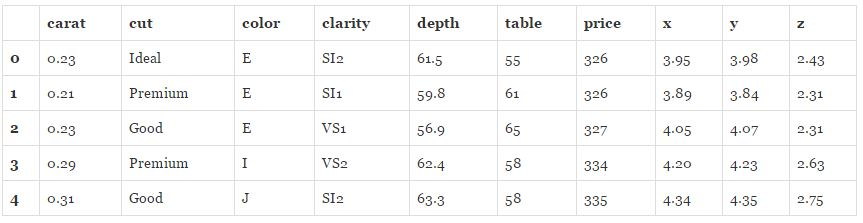
\includegraphics[width=1.1\linewidth]{diamondsdata}

\end{figure}

\end{frame}	
%================================================================================== %
\begin{frame}[fragile]
\frametitle{Aesthetics}
Aesthetics describe how your data will relate to your plots. Some common aesthetics are: x, y, and color. Aesthetics are specific to the type of plot (or layer) you're adding to your visual. For example, a scatterplot (geom\_point) and a line (geom\_line)will share x and y, but only a line chart has a linetype aesthetic.

%For more information about which geoms have which aesthetics, see the DOCS SECTION.
\end{frame}
%================================================================================== %
\begin{frame}[fragile]
\frametitle{Layers}
\begin{itemize}
\item ggplot lets you combine or add different types of visualization components (or layers) together. 
\item I think this is easiest to understand with an example.
\end{itemize}

\end{frame}
%================================================================================== %
\begin{frame}[fragile]
Start with a blank canvas.
\begin{framed}
\begin{verbatim}
p = ggplot(aes(x='date', y='beef'), data=meat)
p
\end{verbatim}
\end{framed}
\begin{figure}
\centering
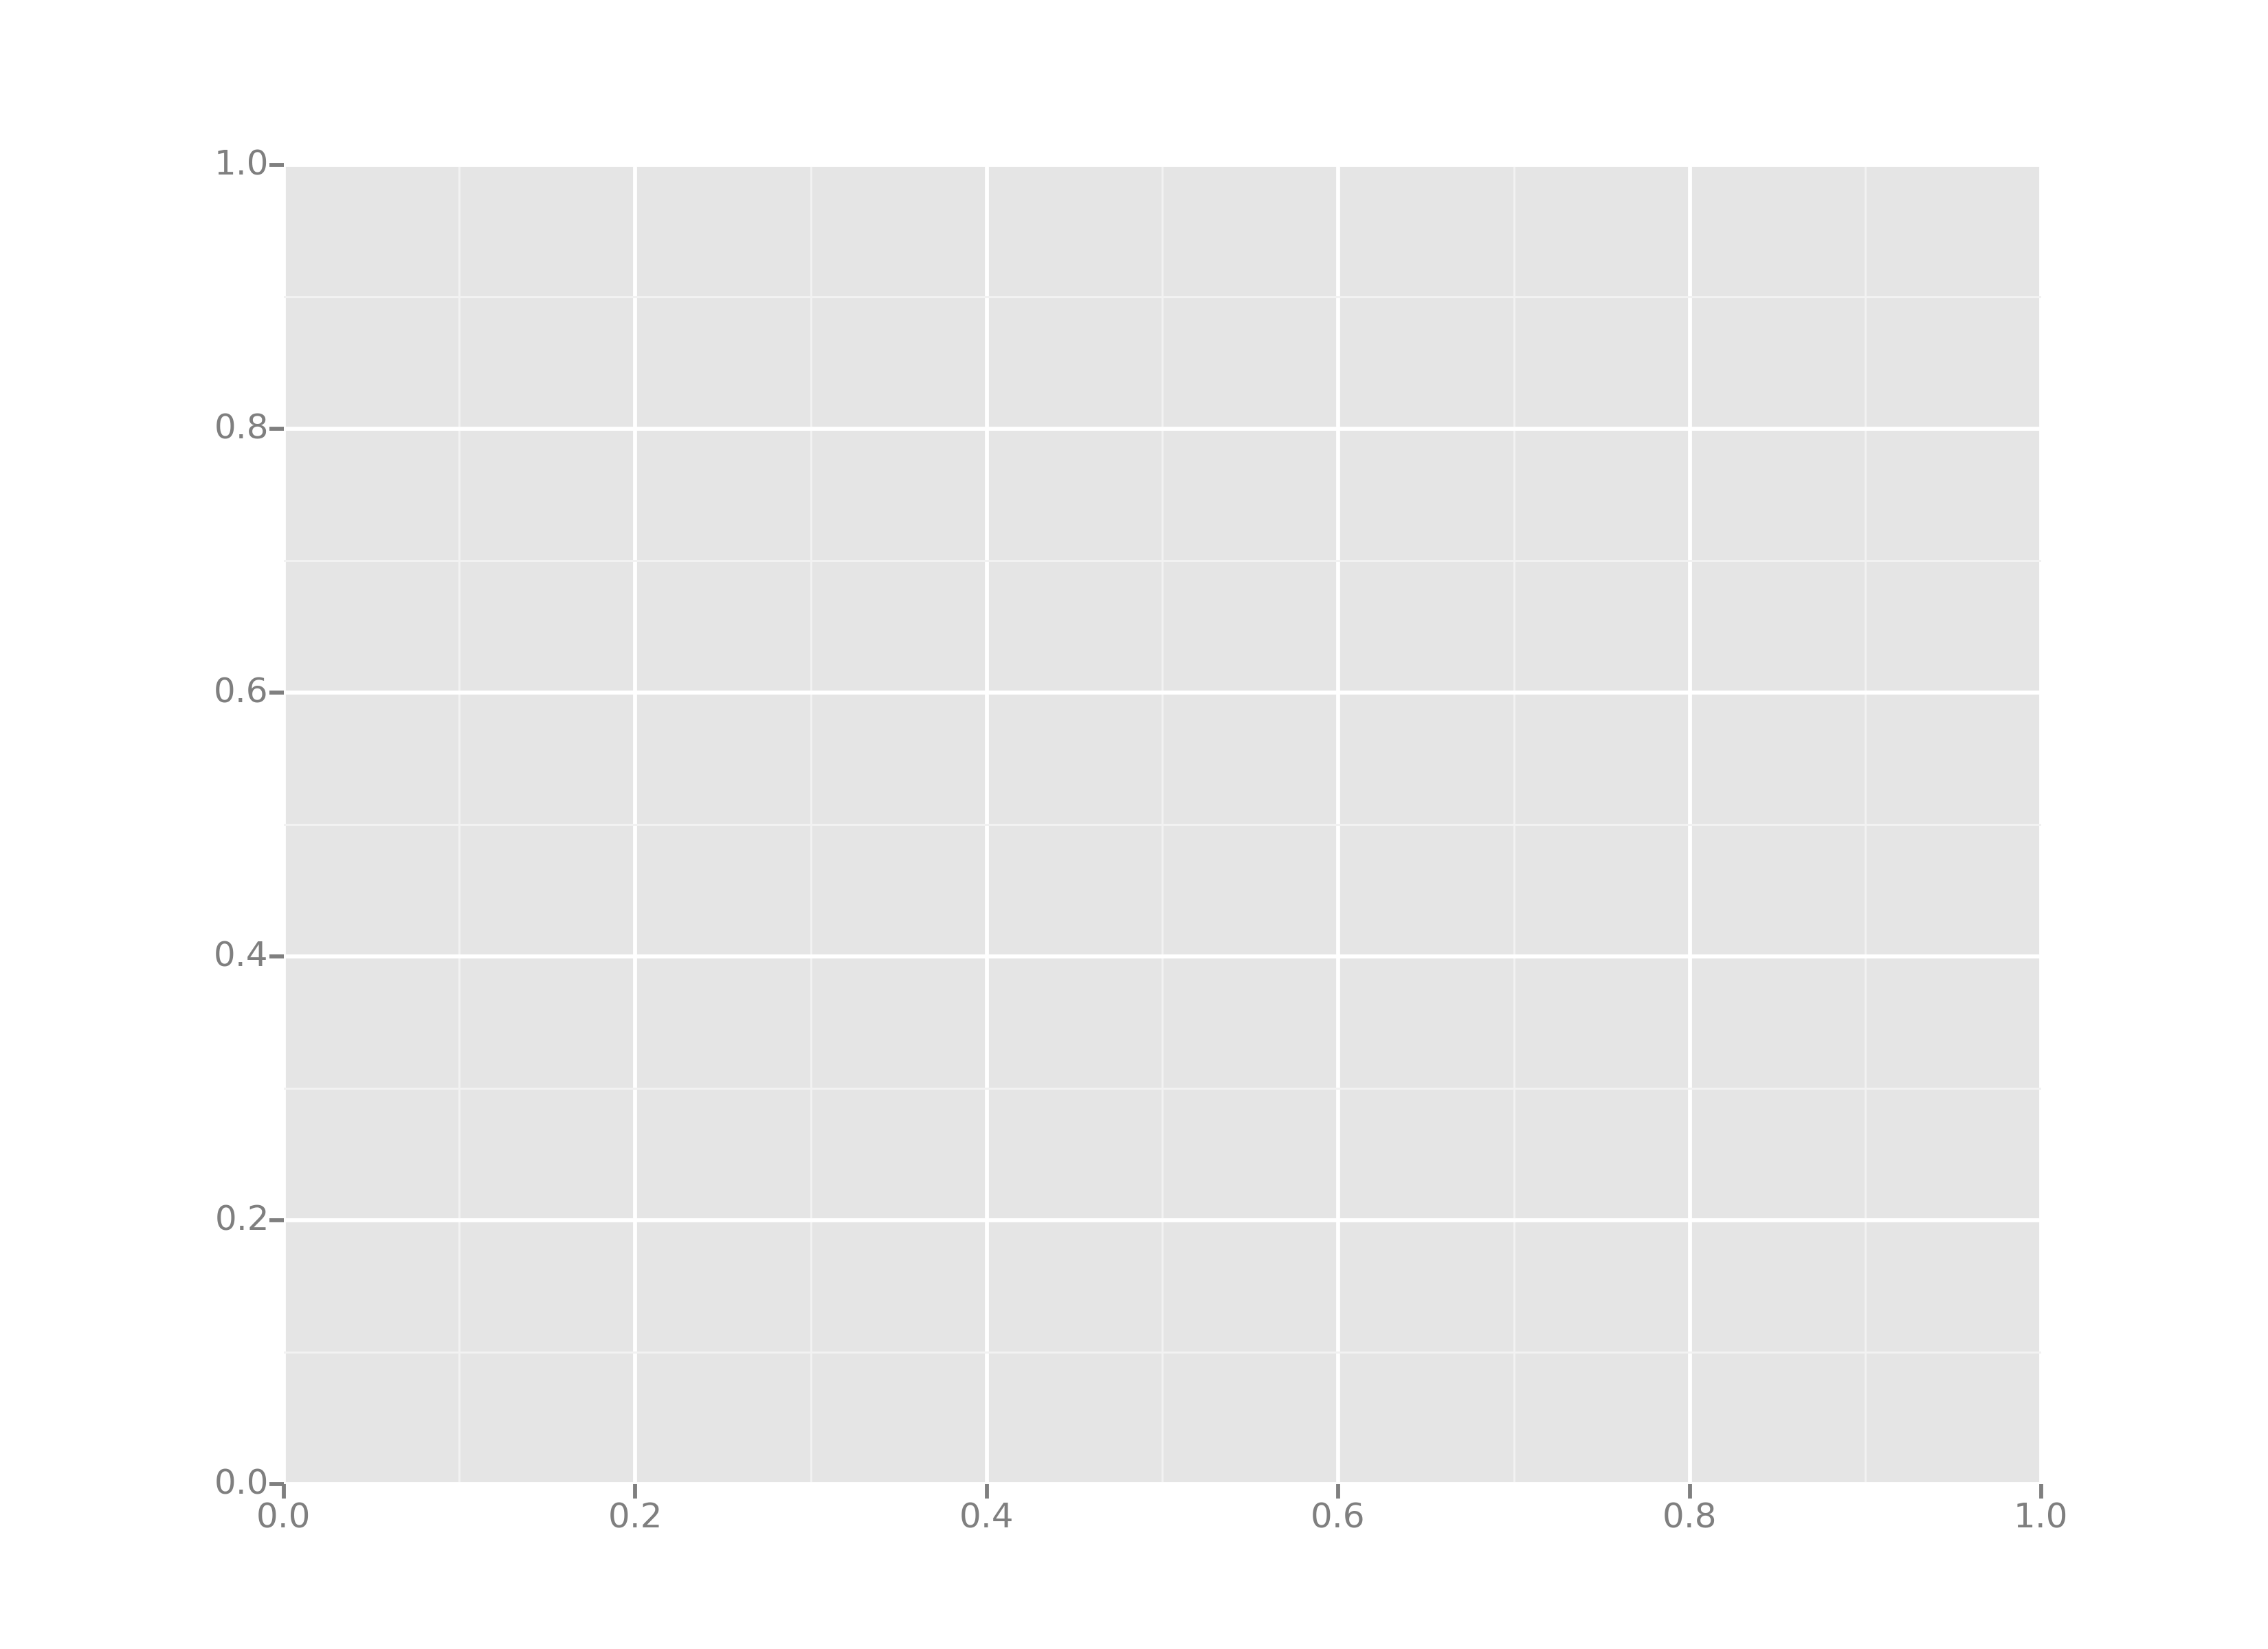
\includegraphics[width=0.7\linewidth]{Layers1}
\caption{}
\label{fig:Layers1}
\end{figure}

\end{frame}
%================================================================================== %
\begin{frame}[fragile]
	Add some points.
	\begin{framed}
		\begin{verbatim}
		p + geom_point()
		\end{verbatim}
	\end{framed}
	\begin{figure}
		\centering
		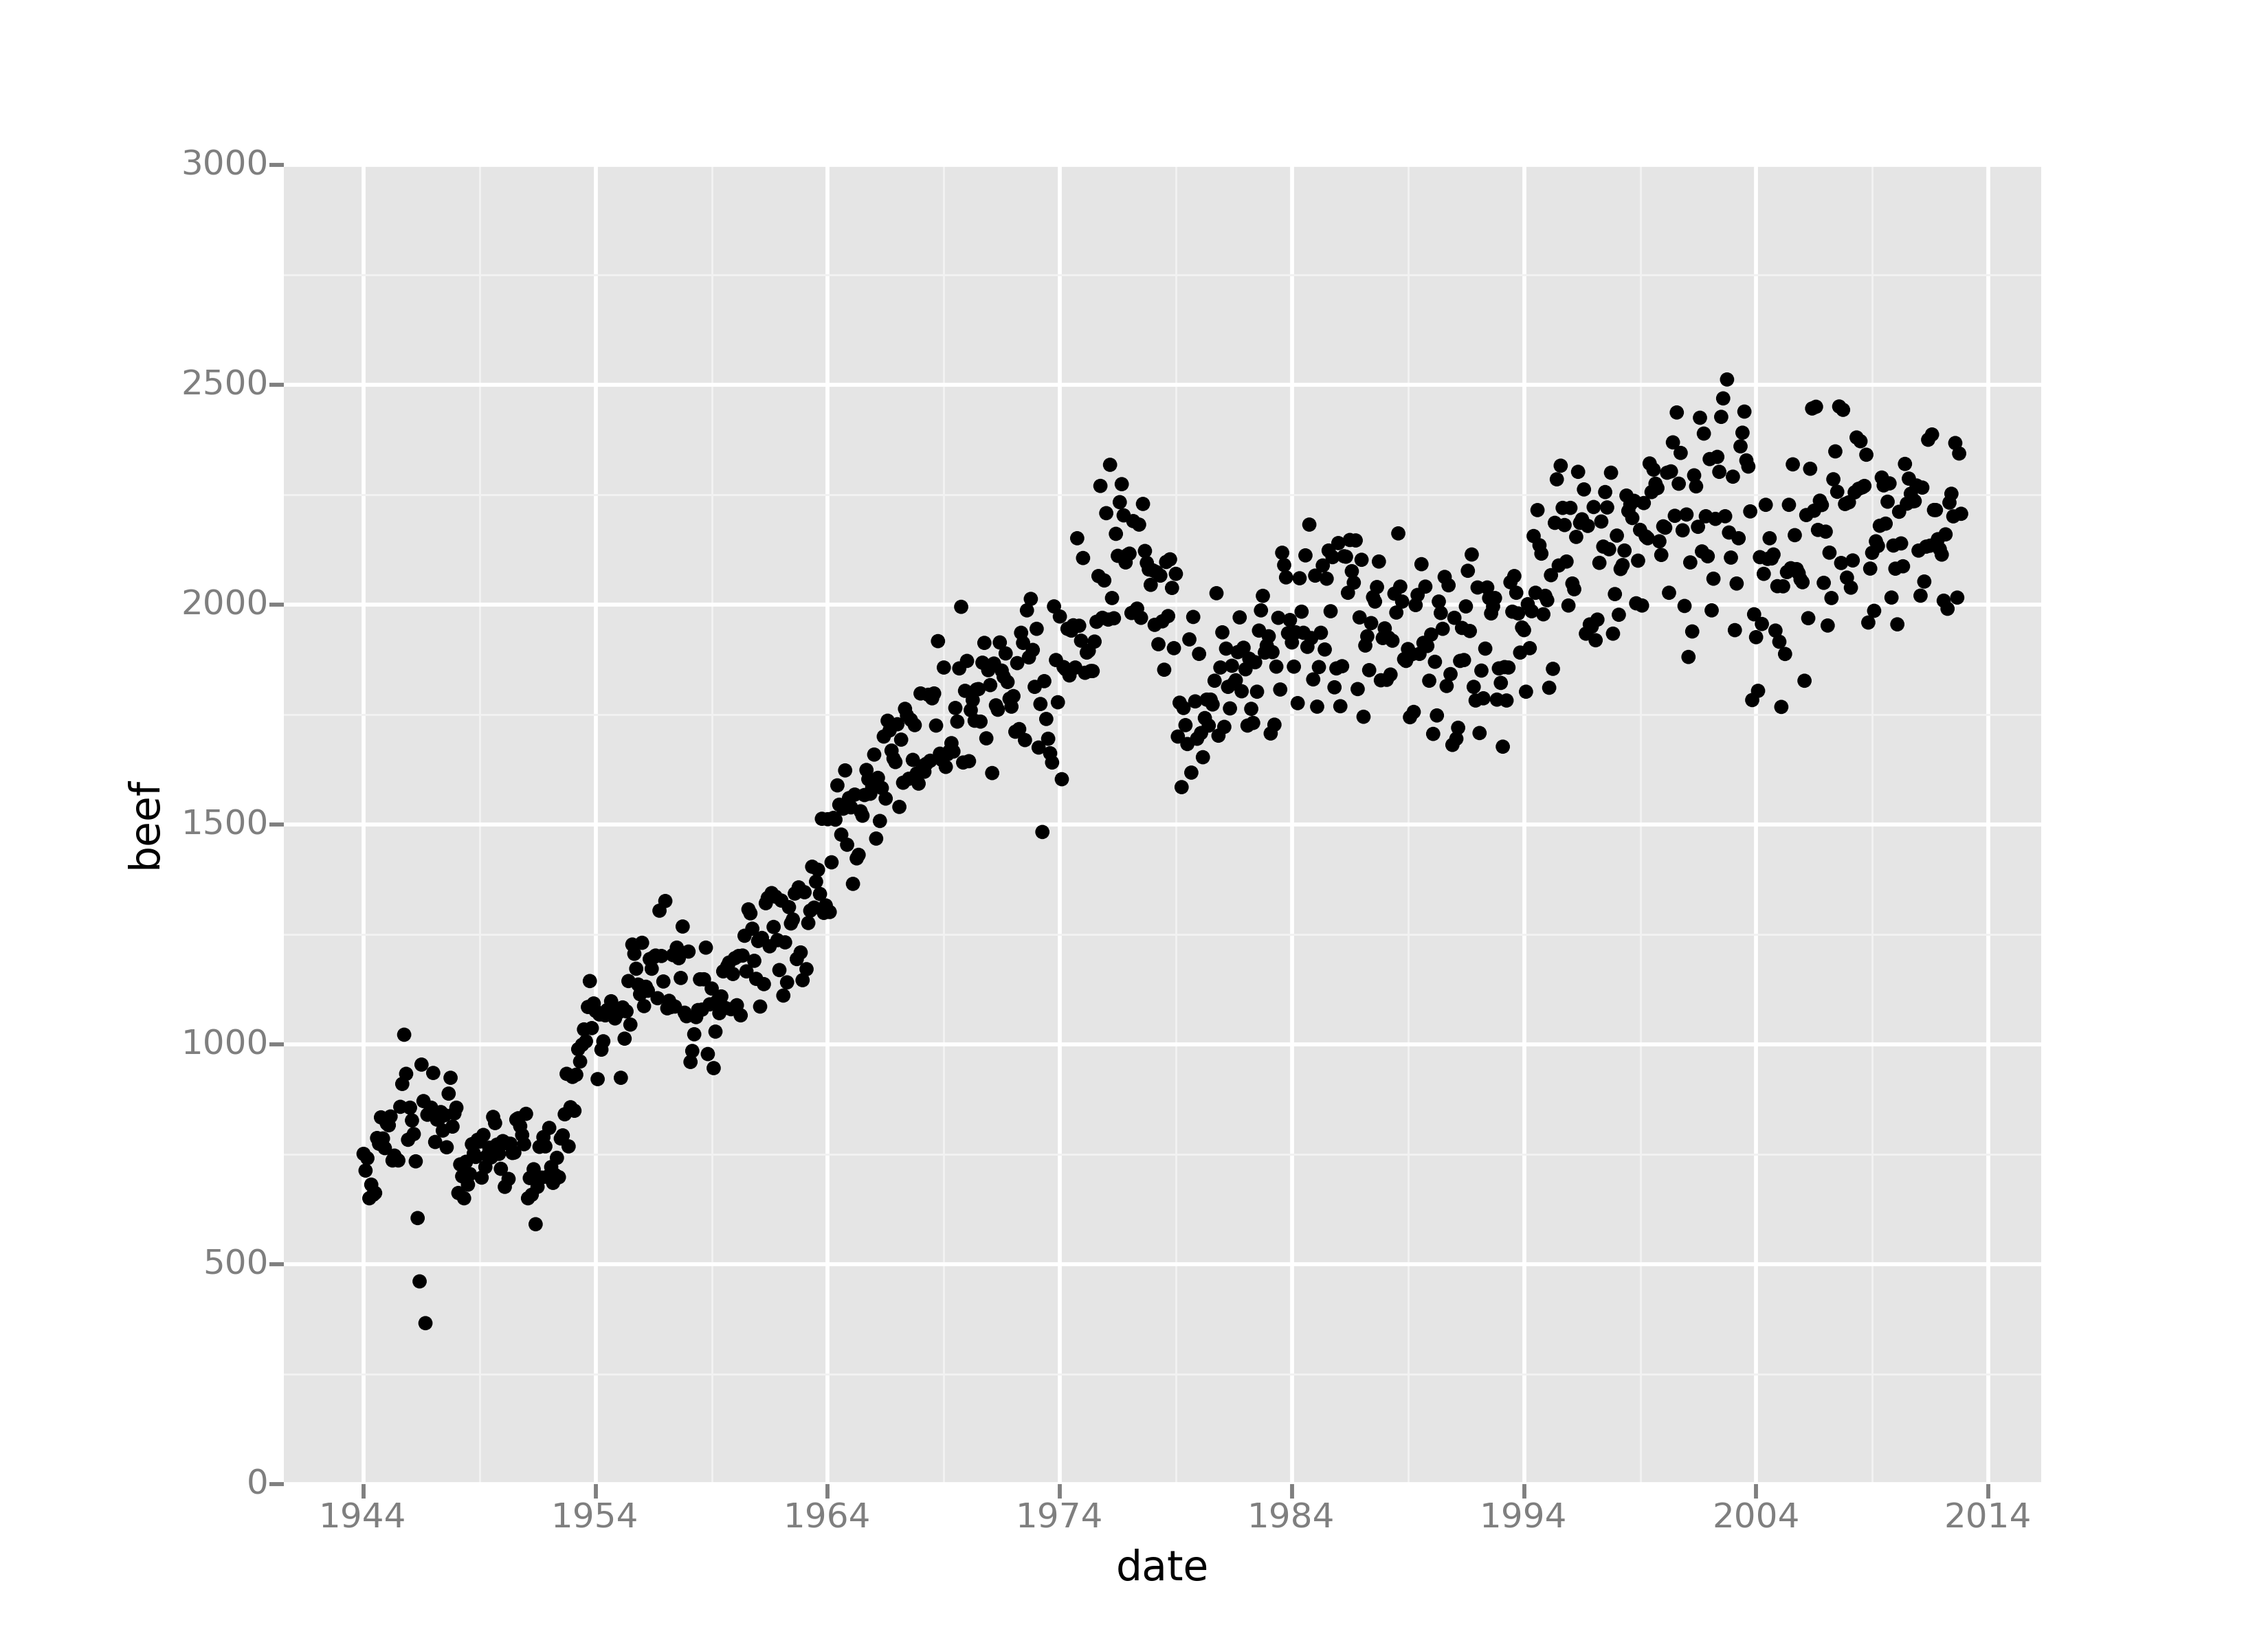
\includegraphics[width=0.7\linewidth]{Layers2}
			\end{figure}
	
	
\end{frame}
\begin{frame}[fragile]
Add a line.
	\begin{framed}
		\begin{verbatim}
p + geom_point() + geom_line()
		\end{verbatim}
	\end{framed}
	\begin{figure}
		\centering
		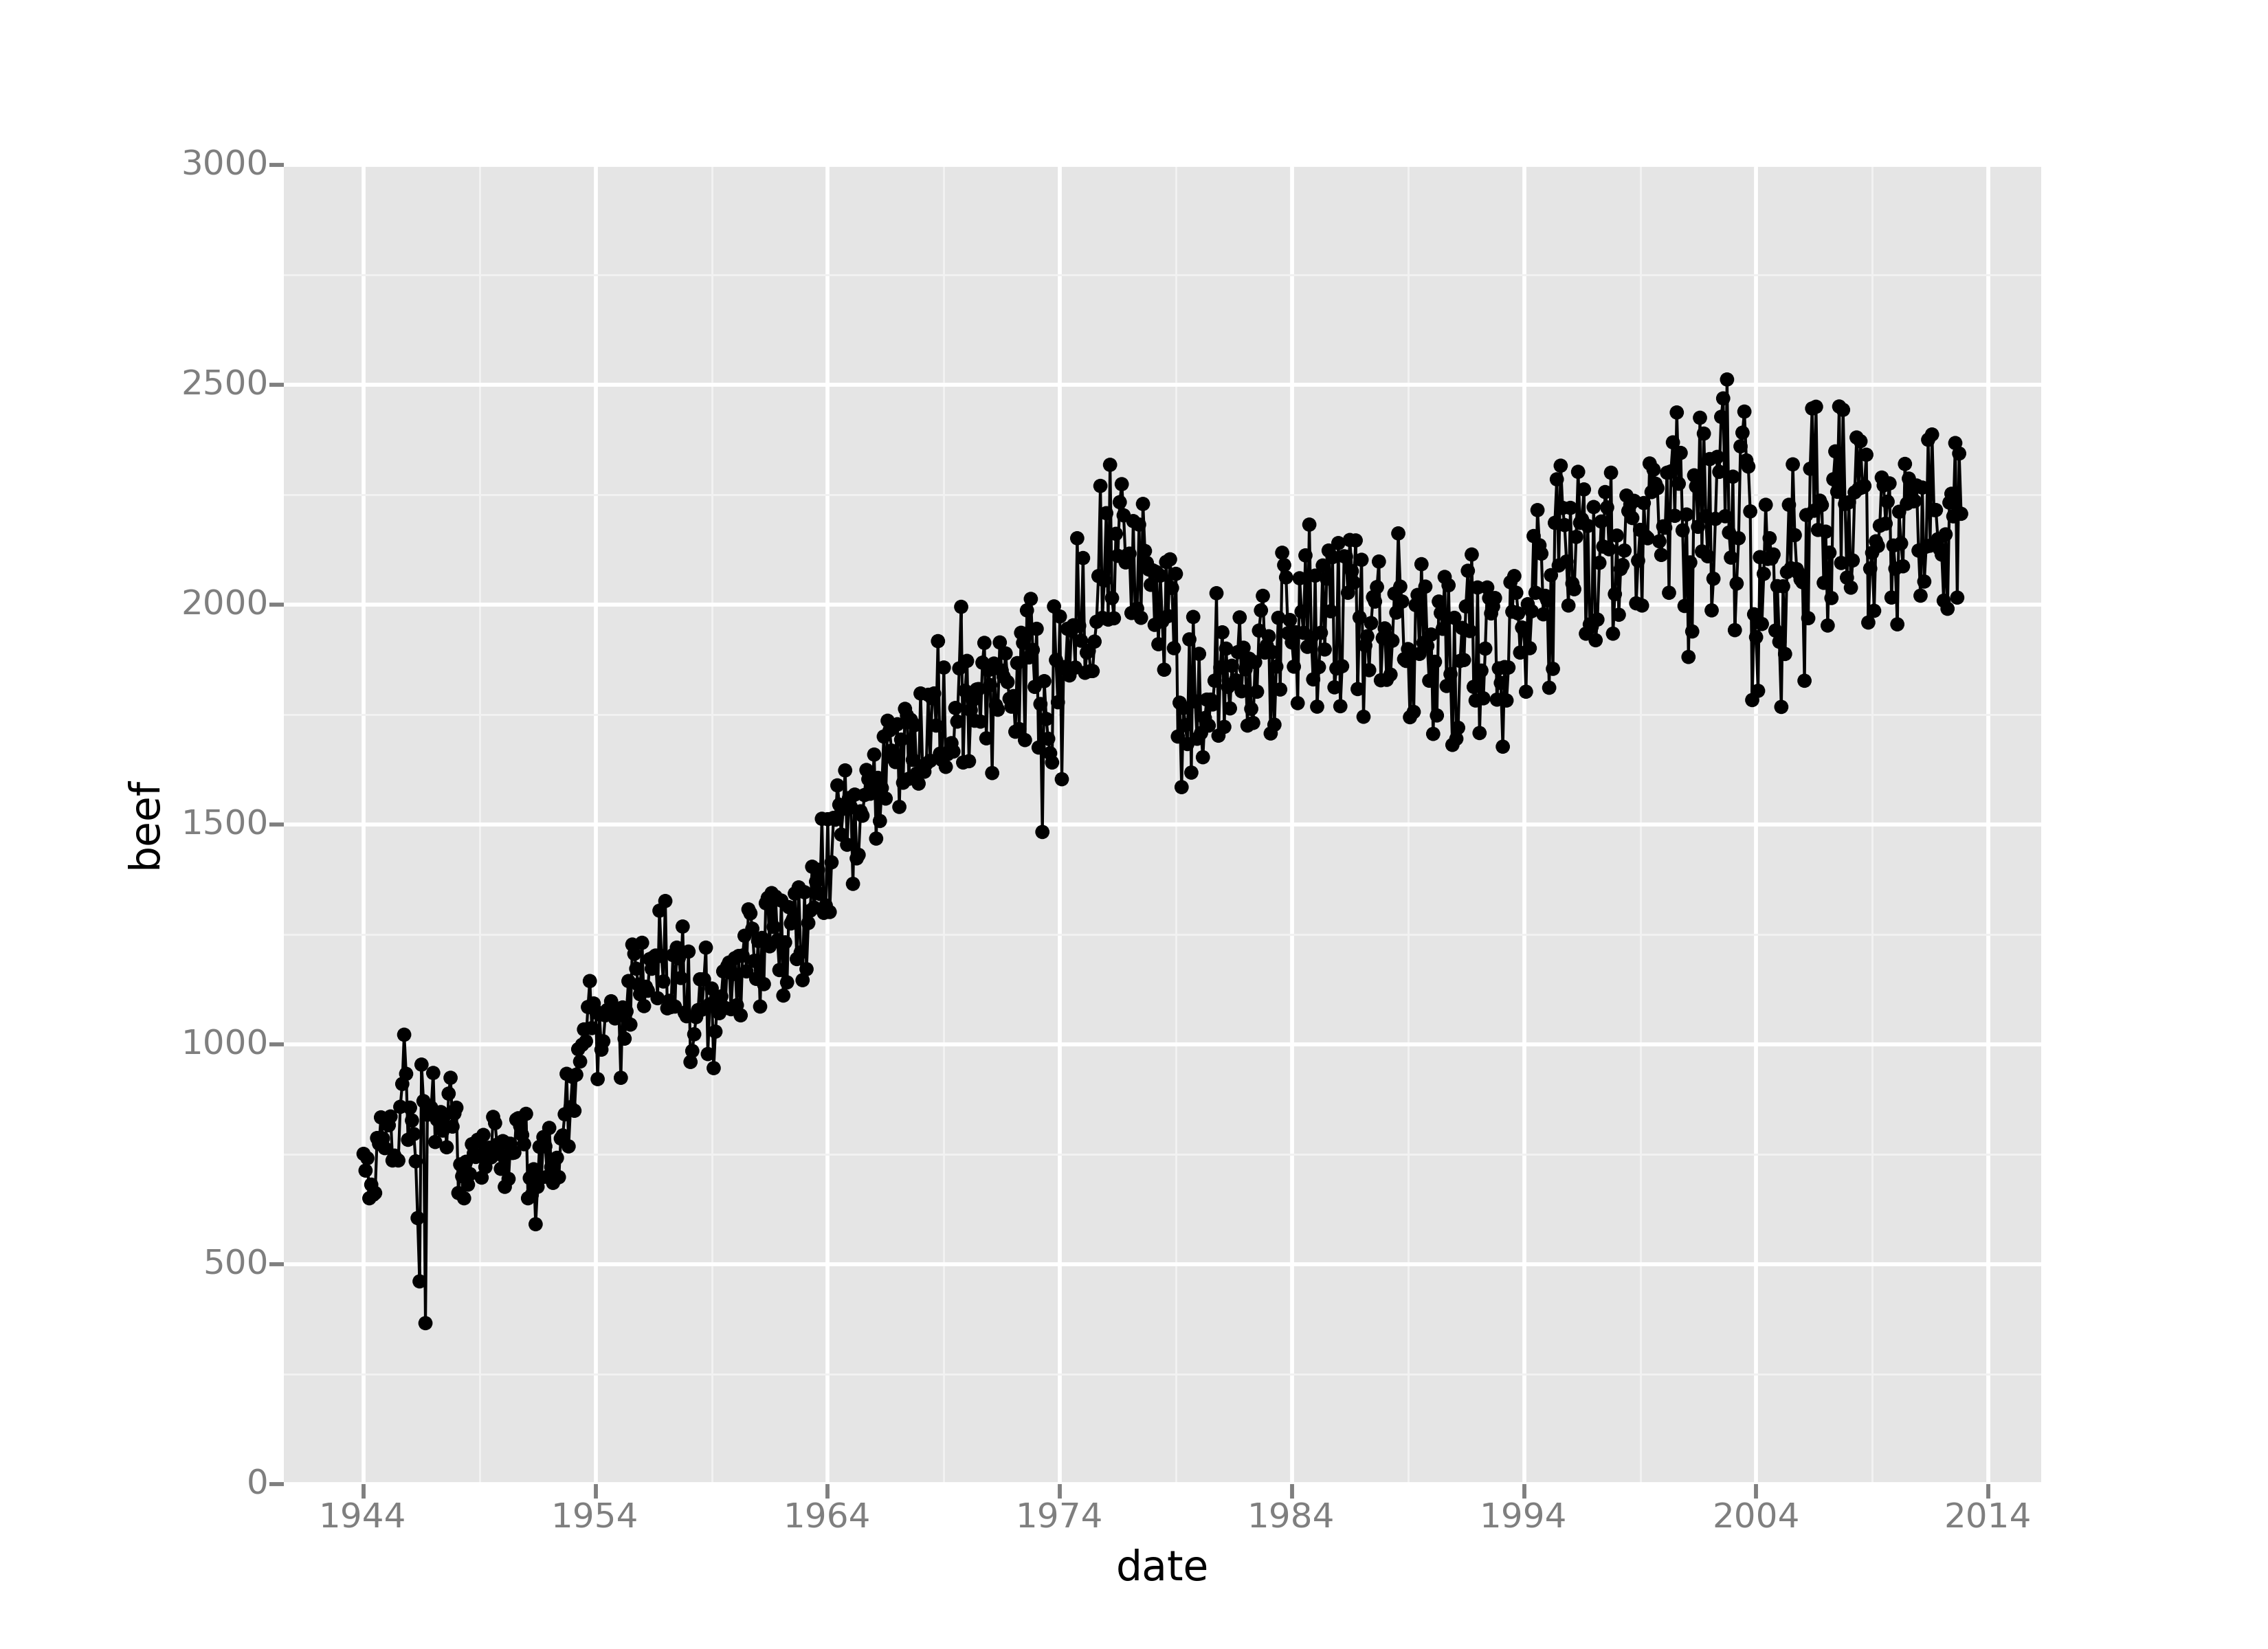
\includegraphics[width=0.7\linewidth]{Layers3}
	\end{figure}
	
	
\end{frame}





%================================================================================== %
\begin{frame}[fragile]
Add a trendline.
	\begin{framed}
\begin{verbatim}
p + geom_point() + geom_line() +
 stat_smooth(color="blue")
\end{verbatim}
\end{framed}
\begin{figure}
\centering
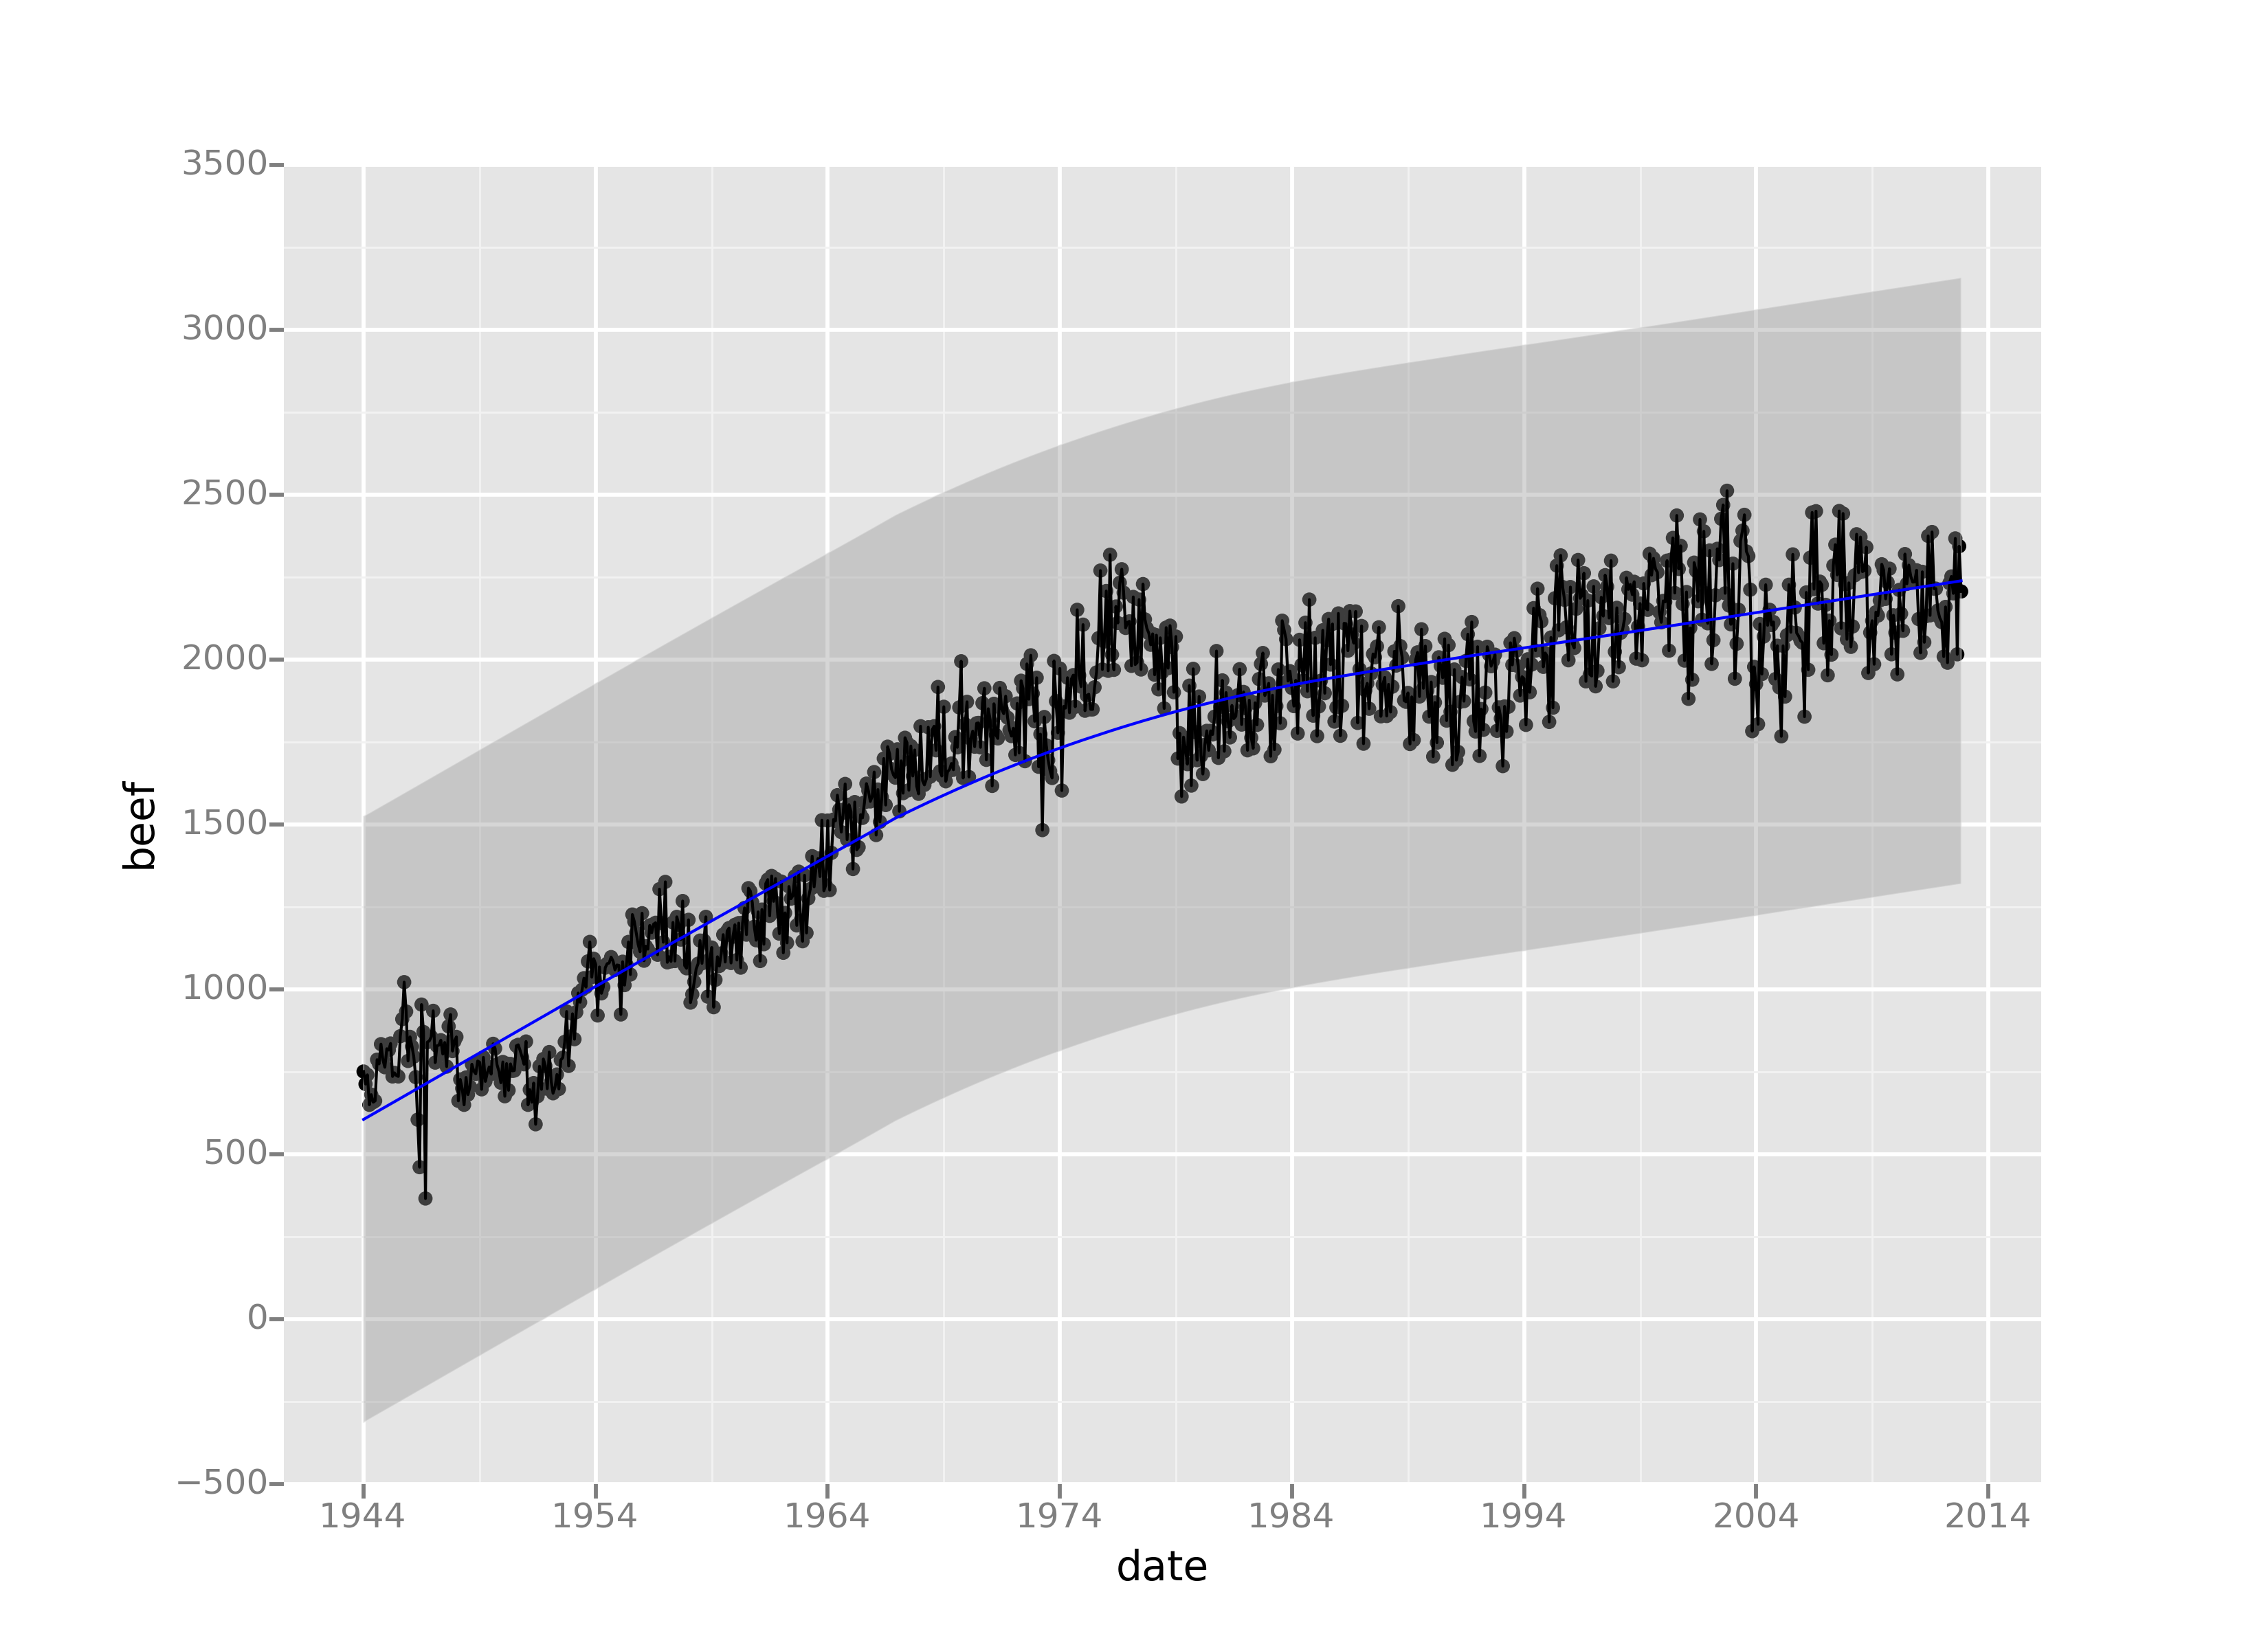
\includegraphics[width=0.7\linewidth]{layers4}
\end{figure}
\end{frame}
%================================================================================== %
\end{document}